\usepackage[latin1]{inputenc}
\usepackage{array}
\usepackage{amsmath}
\usepackage{upgreek}
\usepackage{hyperref}

\usepackage[absolute,overlay]{textpos}

\usepackage{media9}

\setbeamercolor{framesource}{fg=gray}
\setbeamerfont{framesource}{size=\tiny}

\newcommand{\source}[1]{\begin{textblock*}{4cm}(8.7cm,8.6cm)
    \begin{beamercolorbox}[ht=0.5cm,right]{framesource}
        \usebeamerfont{framesource}\usebeamercolor[fg]{framesource} Image Source: {#1}
    \end{beamercolorbox}
\end{textblock*}}

\providecommand{\abs}[1]{\lvert#1\rvert}
\providecommand{\norm}[1]{\lVert#1\rVert}
\providecommand{\dvar}[1]{\, \mathrm{d}#1}
\providecommand{\dx}{\, \dvar{x}}
\providecommand{\dy}{\, \dvar{y}}
\providecommand{\ds}{\, \dvar{s}}
\providecommand{\dt}{\, \dvar{t}}
\providecommand{\du}{\, \dvar{u}}
\providecommand{\dphi}{\, \dvar{u}}
\providecommand{\dtheta}{\, \dvar{\theta}}
\providecommand{\dtau}{\, \dvar{\tau}}
\providecommand{\dr}{\, \dvar{r}}
\providecommand{\dA}{\, \dvar{A}}
% \providecommand{\vint}[2]{\int_{#1} \! #2 \, \mathrm{d}x}
% \providecommand{\sint}[2]{\int_{\partial #1} \! #2 \, \mathrm{d}A}
\renewcommand{\div}{\nabla \cdot}
\providecommand{\shape}{\Omega(p)}
\providecommand{\lagrangian}{\mathcal{L}}
\providecommand{\mesh}{\mathcal{M}}
\providecommand{\boundary}{\partial \shape}
\providecommand{\vint}[1]{\int_{\shape} \! #1 \dx }
\providecommand{\vintd}[2]{\int_{#1} \! #2 \dx }
\providecommand{\sint}[1]{\int_{\boundary} \! #1 \, \dA}
\providecommand{\sintd}[2]{\int_{\partial #1} \! #2 \, \dA}
\providecommand{\pder}[2]{\frac{\partial #1}{\partial #2}}
\providecommand{\tder}[2]{\frac{\mathrm{d} #1}{\mathrm{d} #2}}
\providecommand{\evalat}[2]{\left.#1\right|_{#2}}
\providecommand{\e}{\epsilon}
\newcommand{\defeq}{\vcentcolon=}

% \usepackage{minted}
% \usemintedstyle{perldoc}
% tiny, scriptsize, footnotesize, small, normalsize, large, Large, LARGE,
% huge Huge
% \newminted{d}    {fontsize=\tiny, frame=lines, framesep=1mm}
% \newminted{bash} {fontsize=\tiny, frame=lines, framesep=1mm}
% \newmintedfile{d}{fontsize=\tiny, frame=lines, framesep=1mm}

\usetheme[numbers, compress]{NYU}
% Get rid of the navigation icons
\setbeamertemplate{navigation symbols}{}

\title{Achieving Target Deformations}
\author{}
\date{}
\begin{document}

\begin{frame}
\titlepage
\end{frame}

\section{Introduction}
\begin{frame}{Overview}
Goal: Fabricate shapes with desired deformation properties.

(i.e. The fabricated shape should match the target deformation under a particular
load.)

(Extra challenge: using only one material)
\end{frame}

\begin{frame}
\begin{figure}
\includegraphics[width=0.7\textwidth]{Images/material_opt_bump_half.png}

\vspace{3mm}
\includegraphics[width=0.7\textwidth]{Images/microstructure_bump_half_box.png}
\end{figure}

\begin{enumerate}
\item Find material properties that achieves the goal.
\item Find geometry that achieves these material properties.
\end{enumerate}
\end{frame}

\section{Material Optimization}

\begin{frame}{1D Example}
\begin{figure}
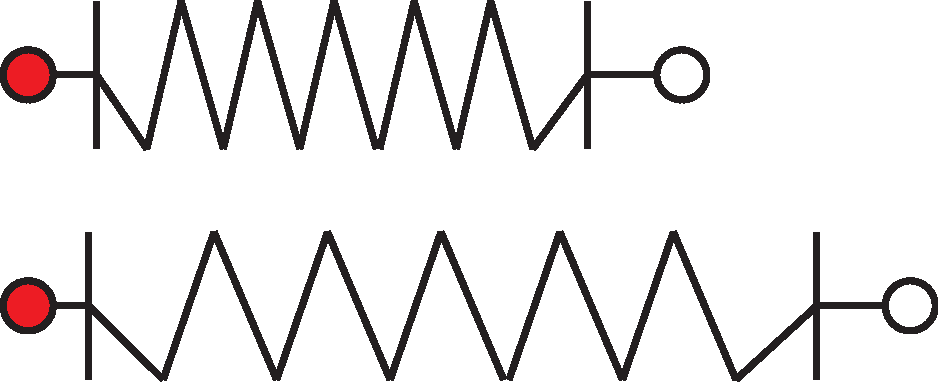
\includegraphics[width=0.6\textwidth]{Images/spring_stretch.pdf}
\end{figure}

\begin{itemize}
\item Hook's law: $F = -k u$
\pause \item In 1D, Force $F$ and displacement $u$ are coupled through spring constant $k$.
\pause \item In 3D, stress $\sigma$ and strain $\epsilon$ are coupled through
material tensor.
\end{itemize}
\end{frame}

\begin{frame}{Discretize material properties}
\begin{figure}
\hspace{\fill}
\includegraphics[width=0.45\textwidth]{Images/material_opt_half_period.png}
\hspace{\fill}
\includegraphics[width=0.45\textwidth]{Images/material_opt_full_period.png}
\hspace{\fill}

\vspace{3mm}
\hspace{\fill}
\includegraphics[width=0.45\textwidth]{Images/material_opt_bump_half.png}
\hspace{\fill}
\includegraphics[width=0.45\textwidth]{Images/material_opt_bump_third.png}
\hspace{\fill}
\end{figure}

\begin{itemize}
\item Homogeneous material properties is very restrictive.
Heterogeneous material is needed to achieve interesting examples.
\end{itemize}
\end{frame}

\begin{frame}{Material optimization}
\begin{align*}
\min_{E, \nu} & \int_{\partial \Omega} \|u - u^*\|^2 \dA\\
\textrm{s.t.} & \nabla \cdot \sigma(u) = f \qquad \forall x \in \Omega\\
& \sigma(u) \cdot n = t \qquad \forall x \in \partial \Omega_{N}
\end{align*}
where $E,\nu : \Omega \to \mathbb{R}$.

\begin{itemize}
\pause \item The optimal solution is not unique.
\pause \item The constraint is a PDE.
\end{itemize}
\end{frame}

\begin{frame}{What we have tried?}
\begin{itemize}
\item Gradient-based algorithm: gradient descent, BFGS.
\item A local/global iteration algorithm.
\begin{itemize}
\item Compute strain with only Dirichlet BC enforced.
\item Compute stress with only Neumann BC enforced.
\item Fit material properties using constrained nonlinear least sqaure.
\end{itemize}
\end{itemize}
\end{frame}

\begin{frame}{Results}
\begin{figure}
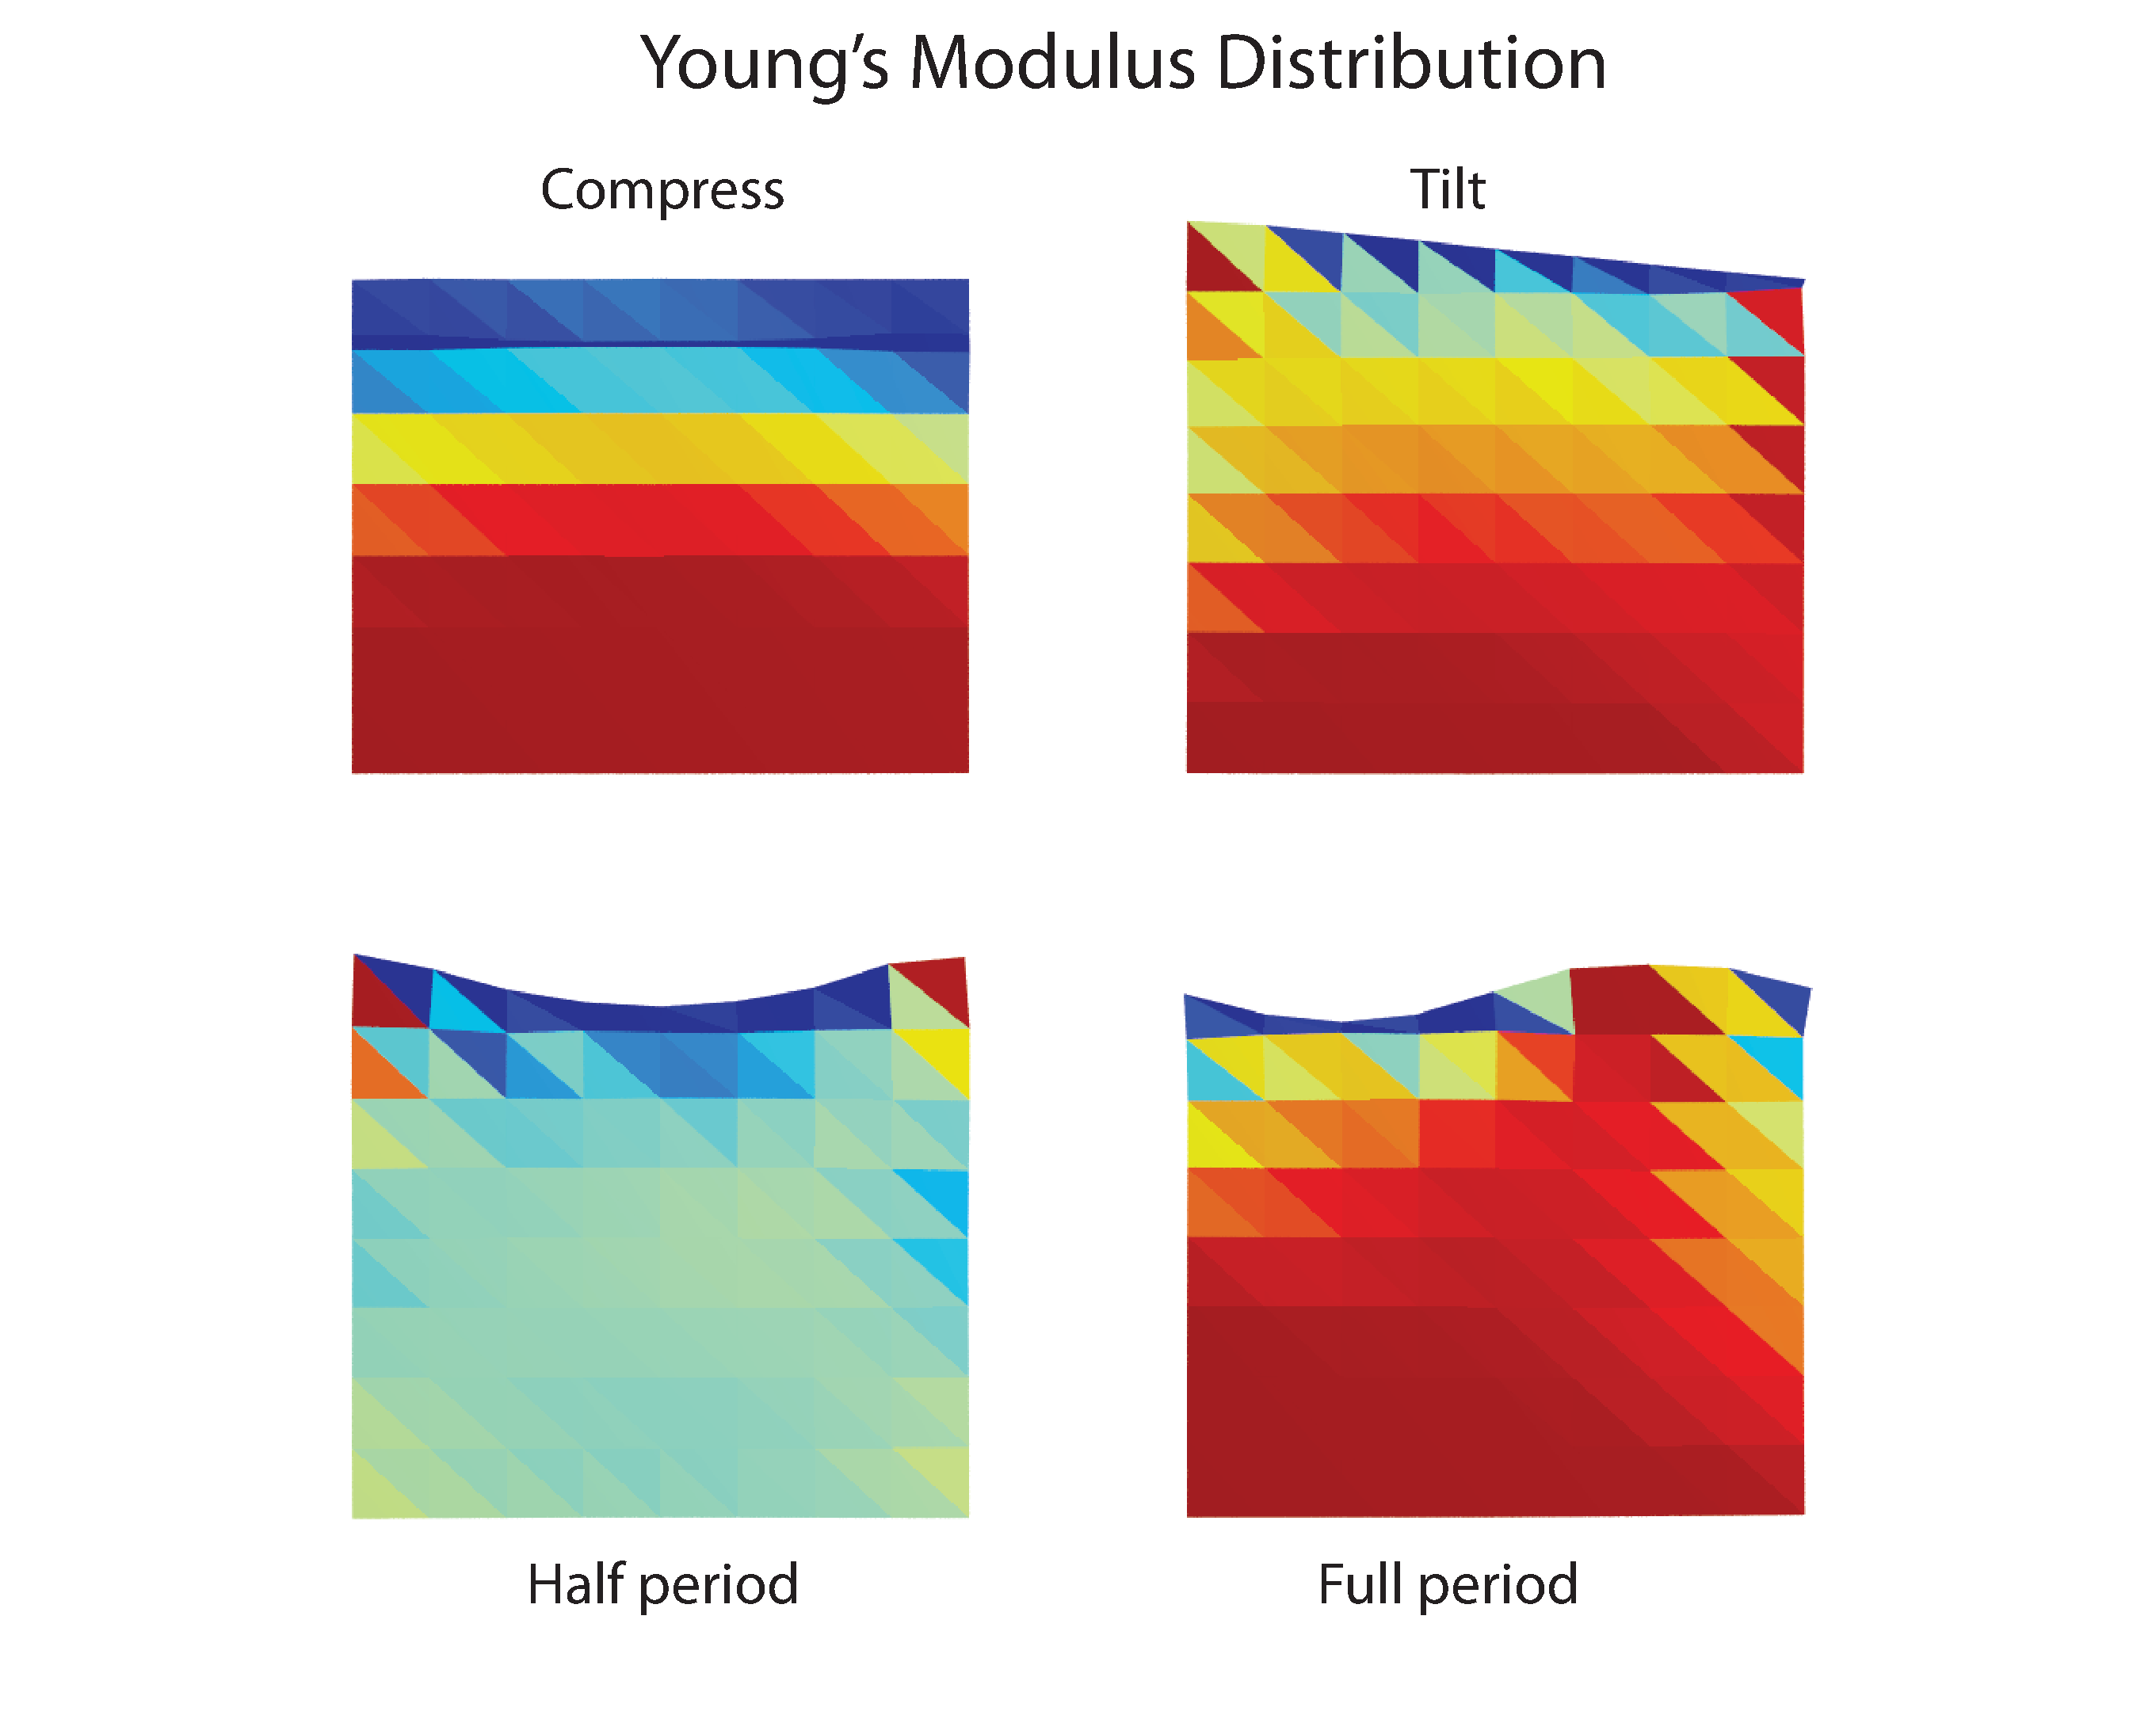
\includegraphics[width=0.9\textwidth]{Images/box_compression_test.pdf}
\end{figure}

\end{frame}



\section{Homogenization}
\begin{frame}{Variable Properties With a Single Material}
    \begin{itemize}
        \item How can we vary the material properties with one material? Vary the microstructure
              geometry.
        \pause 
        \begin{figure}
            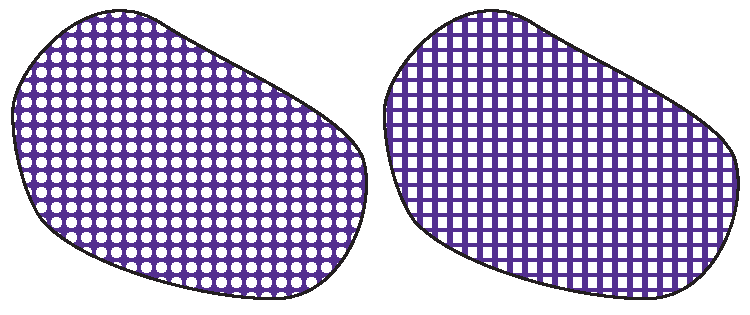
\includegraphics[width=.65\textwidth]{Images/two_patterns.pdf}
        \end{figure}
        \pause \item Gives different effective, ``homogenized,'' material properties:
        \begin{figure}
            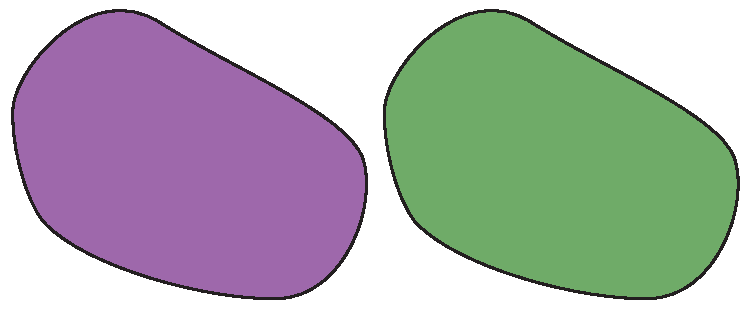
\includegraphics[width=.65\textwidth]{Images/two_materials.pdf}
        \end{figure}
    \end{itemize}
\end{frame}

\begin{frame}{Homogenized Elasticity Tensor}
    \begin{itemize}
\item Recall: material properties (elasticity tensor) tell us how strain maps to
    stress.
\item Intuitively: homogenized elasticity tensor tells us how the {\bf average} strain
    ``around'' a point maps to the {\bf average} stress.
\item Can't spatially average the properties!
    \begin{figure}
        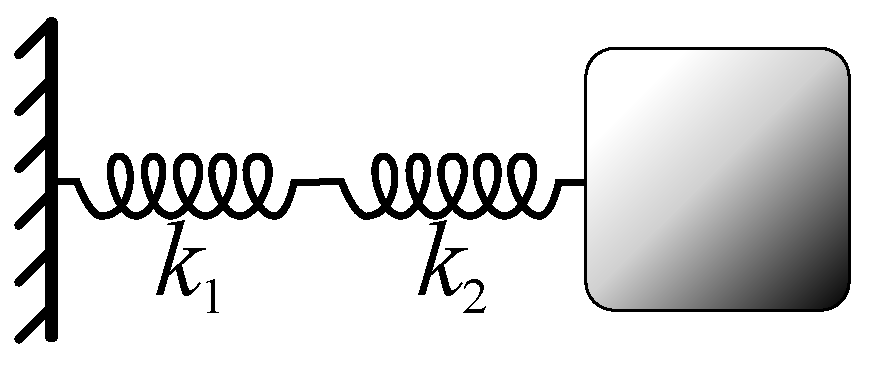
\includegraphics[width=.50\textwidth]{Images/SpringsInSeriesWiki.pdf}
    \end{figure}
    $$k^H = \frac{1}{\frac{1}{k_1} + \frac{1}{k_2}} \ne \frac{1}{2}\left(k_1 +
    k_2\right)$$
    \end{itemize}
\end{frame}

\begin{frame}{Homogenized Elasticity Tensor}
    \begin{itemize}
        \item To use nice mathematical tools (periodic homogenization), restrict
            to microstructures given by tiled base cells. 
            \begin{figure}
                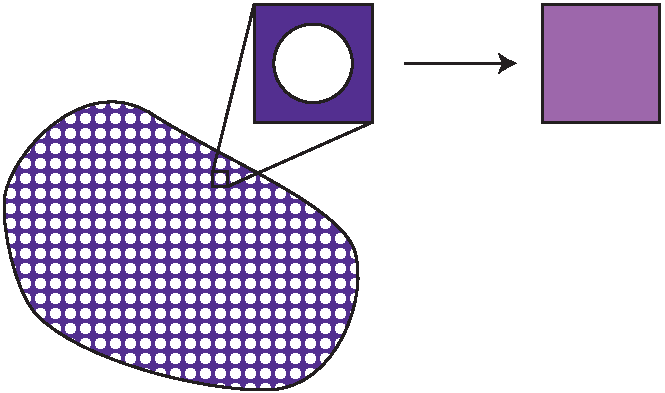
\includegraphics[width=.50\textwidth]{Images/cell_homogenize.pdf}
                \includegraphics[width=.40\textwidth]{Images/base.png}
            \end{figure}
        \item General idea: for all possible average strains over the cell, compute the
              average stress.
    \end{itemize}
\end{frame}

\begin{frame}{Strain Tensor Basis}
    \begin{itemize}
        \item Linearity of stress-strain relationship saves us: we only need to consider 3
    ``basis strain tensors'' in 2D: 2 axis-aligned stretches and 1 shear.
    \begin{figure}
        \includegraphics[width=.25\textwidth]{Images/cstrain_x.png}
        \includegraphics[width=.25\textwidth]{Images/cstrain_y.png}
        \includegraphics[width=.25\textwidth]{Images/cstrain_shear.png}
    \end{figure}
    \begin{figure}
        \includegraphics[width=.25\textwidth]{Images/disp_x.png}
        \includegraphics[width=.25\textwidth]{Images/disp_y.png}
        \includegraphics[width=.25\textwidth]{Images/disp_shear.png}
    \end{figure}
    \end{itemize}
\end{frame}

\begin{frame}{Computing the Homogenized Elasticity Tensor}
    \begin{figure}
        \includegraphics[width=.25\textwidth]{Images/disp_x.png}
        \includegraphics[width=.25\textwidth]{Images/disp_y.png}
        \includegraphics[width=.25\textwidth]{Images/disp_shear.png}
    \end{figure}
    \begin{itemize}
        \item For each constant strain basis tensor:
        \begin{itemize}
            \item Impose the average constant strain and compute how the geometry
                  actually deforms
            \item Average the stress tensor over the cell
            \item Store flattened average stress tensor in a column of the
                  flattened elasticity tensor.
        \end{itemize}
    \end{itemize}
\end{frame}

\begin{frame}{Computing the Homogenized Elasticity Tensor}
    \begin{figure}
        
\includegraphics[width=.20\textwidth]{Images/cell.pdf}
    \end{figure}
    \begin{align*}
         -\nabla \cdot (C^\text{base} : [e({\bf w}^{ij}) + e^{ij}]) = {\bf 0} & \quad \text{in } \omega \\
    {\bf \hat n} \cdot (C^\text{base} : [e({\bf w}^{ij}) + e^{ij}]) = {\bf 0} & \quad \text{on } \partial \omega \setminus \partial Y \\
        {\bf w}^{ij}({\bf y})\ Y \text{-periodic} & \\
        \int_\omega \! {\bf w}^{ij}({\bf y})  \, \mathrm{d} {\bf y} =  {\bf 0}, 
    \end{align*}
    \begin{equation*}
        \label{eqn:Eh}
    C^H_{ijkl} = \frac{1}{|Y|} \int_Y C^\text{base}_{ijpq} [e({\bf w}^{kl})] + e^{ij}]_{pq} \, \mathrm{d} {\bf y}
    \end{equation*}
    \begin{itemize}
        \pause \item As cell size shrinks to zero, the microstructure simulation
            converges to a homogenous simulation with $C^H$
   \end{itemize}
\end{frame}

\section{Patterns}

\begin{frame}{Wire-based microstructures}
% Large examples of wire-based microstructure
\begin{figure}
\includegraphics[width=0.8\textwidth]{Images/diamond_cube.png}
\end{figure}
\end{frame}

\begin{frame}{Wire-based microstructures}
% motivation of using wire-based structures.
\begin{figure}
\centering
\hspace{\fill}
\includegraphics[width=0.4\textwidth]{Images/molecular_structures.png}
\hspace{\fill}
\pause \includegraphics[width=0.4\textwidth]{Images/javits_center.png}
\hspace{\fill}

\vspace{3mm}
\pause \includegraphics[width=0.9\textwidth]{Images/sponge_structure.pdf}
\end{figure}
\end{frame}

\begin{frame}{Single cell patterns}
% Show a few single cell patterns
% brick5, diamond, star, truncated octahedron
\begin{figure}
\hspace{\fill}
\includegraphics[width=0.4\textwidth]{Images/brick5_cell.png}
\hspace{\fill}
\includegraphics[width=0.4\textwidth]{Images/star_cell.png}
\hspace{\fill}

\vspace{3mm}
\hspace{\fill}
\includegraphics[width=0.4\textwidth]{Images/truncated_octahedron_cell.png}
\hspace{\fill}
\includegraphics[width=0.4\textwidth]{Images/diamond_cell.png}
\hspace{\fill}
\end{figure}
\end{frame}

\begin{frame}{Single cell patterns}
% Show a few single cell patterns
% brick5, diamond, star, truncated octahedron
\begin{figure}
\hspace{\fill}
\includegraphics[width=0.4\textwidth]{Images/brick5_cell_source.png}
\hspace{\fill}
\includegraphics[width=0.4\textwidth]{Images/star_cell_source.png}
\hspace{\fill}

\vspace{3mm}
\hspace{\fill}
\includegraphics[width=0.4\textwidth]{Images/truncated_octahedron_cell_source.png}
\hspace{\fill}
\includegraphics[width=0.4\textwidth]{Images/diamond_cell_source.png}
\hspace{\fill}
\end{figure}
\end{frame}

\begin{frame}{Inflation}
% Illustrate the steps
\begin{figure}
\centering
\hspace{\fill}
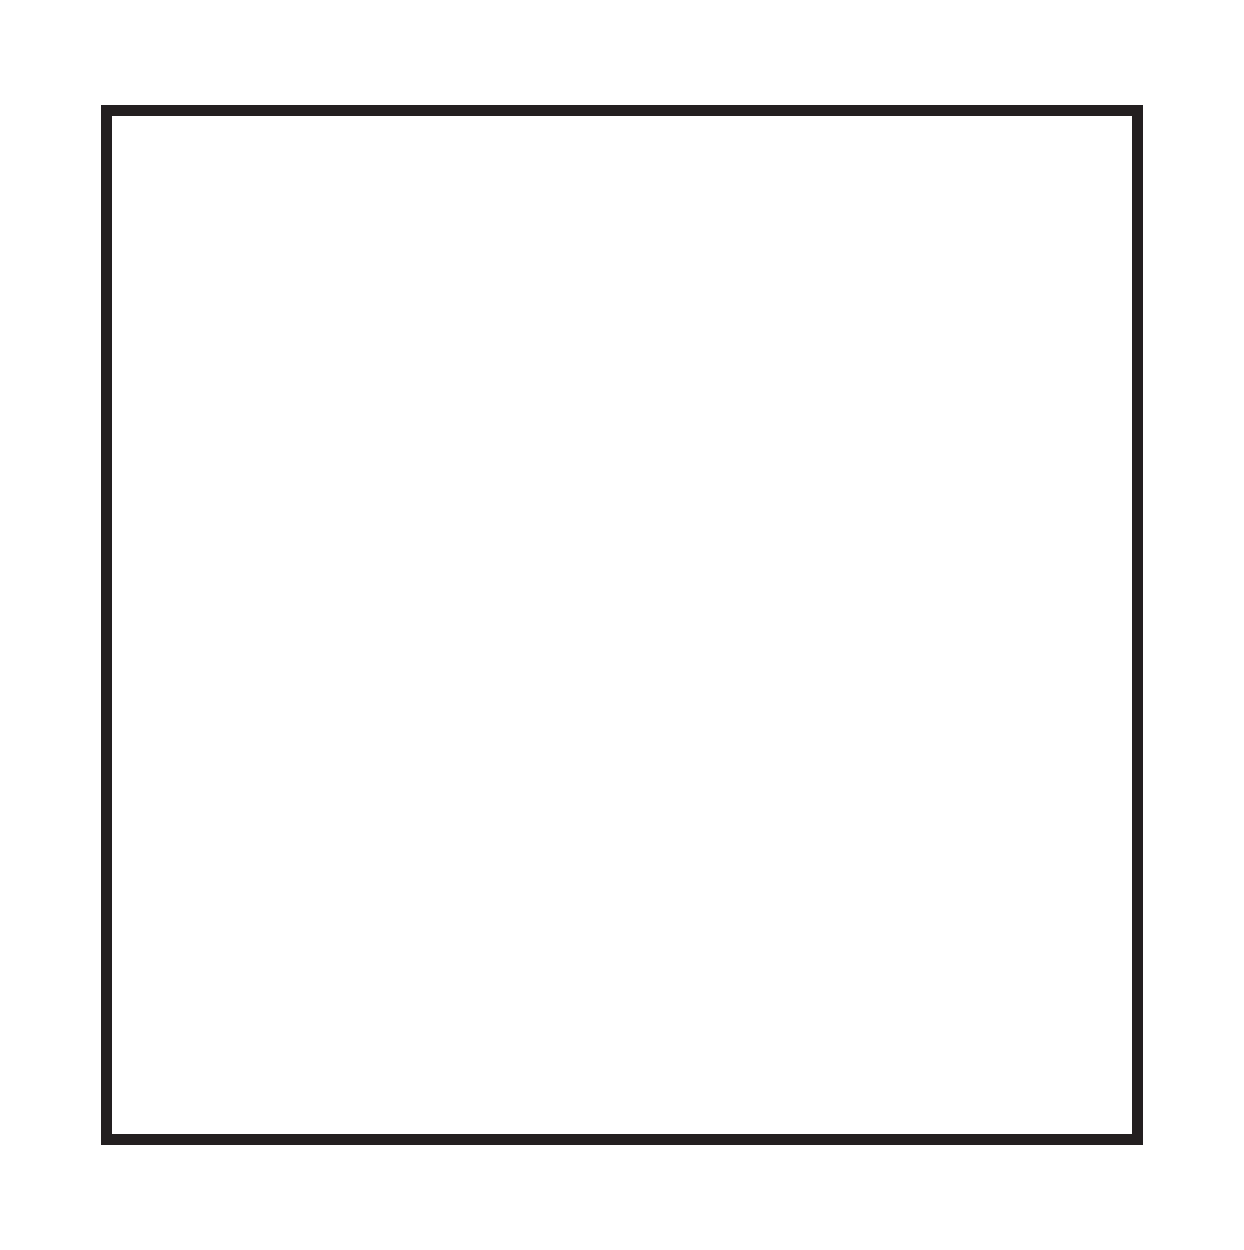
\includegraphics[width=0.3\textwidth]{Images/inflation_0.pdf}
\hspace{\fill}
\pause 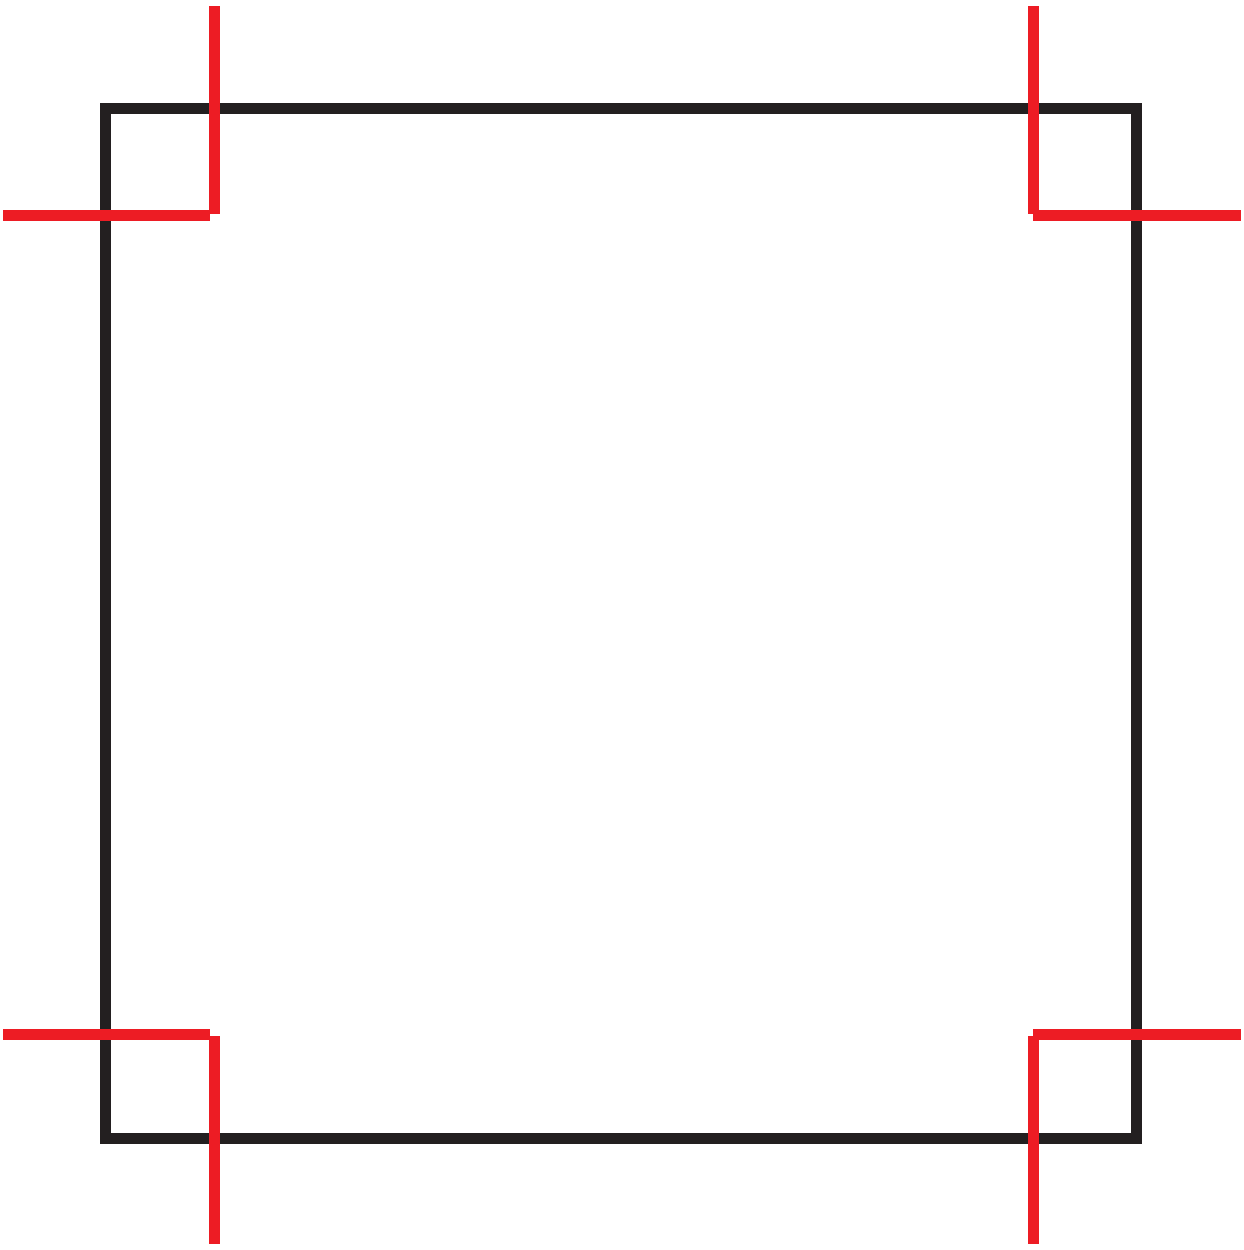
\includegraphics[width=0.3\textwidth]{Images/inflation_1.pdf}
\hspace{\fill}
\pause 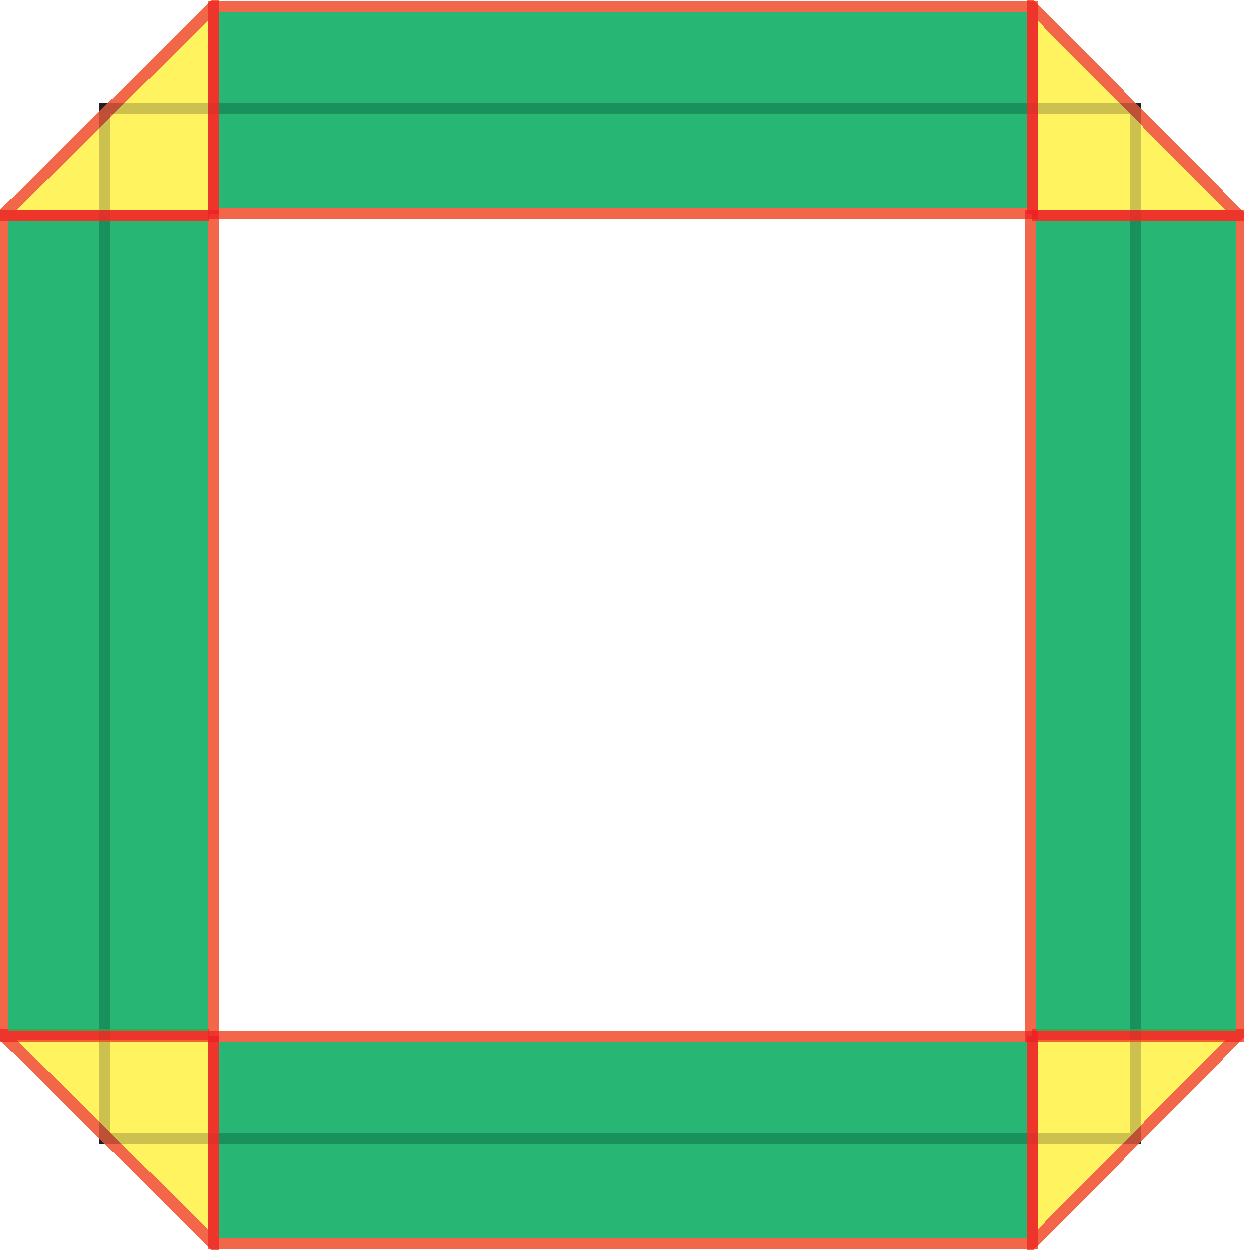
\includegraphics[width=0.3\textwidth]{Images/inflation_2.pdf}
\hspace{\fill}

\vspace{3mm}
\hspace{\fill}
\pause 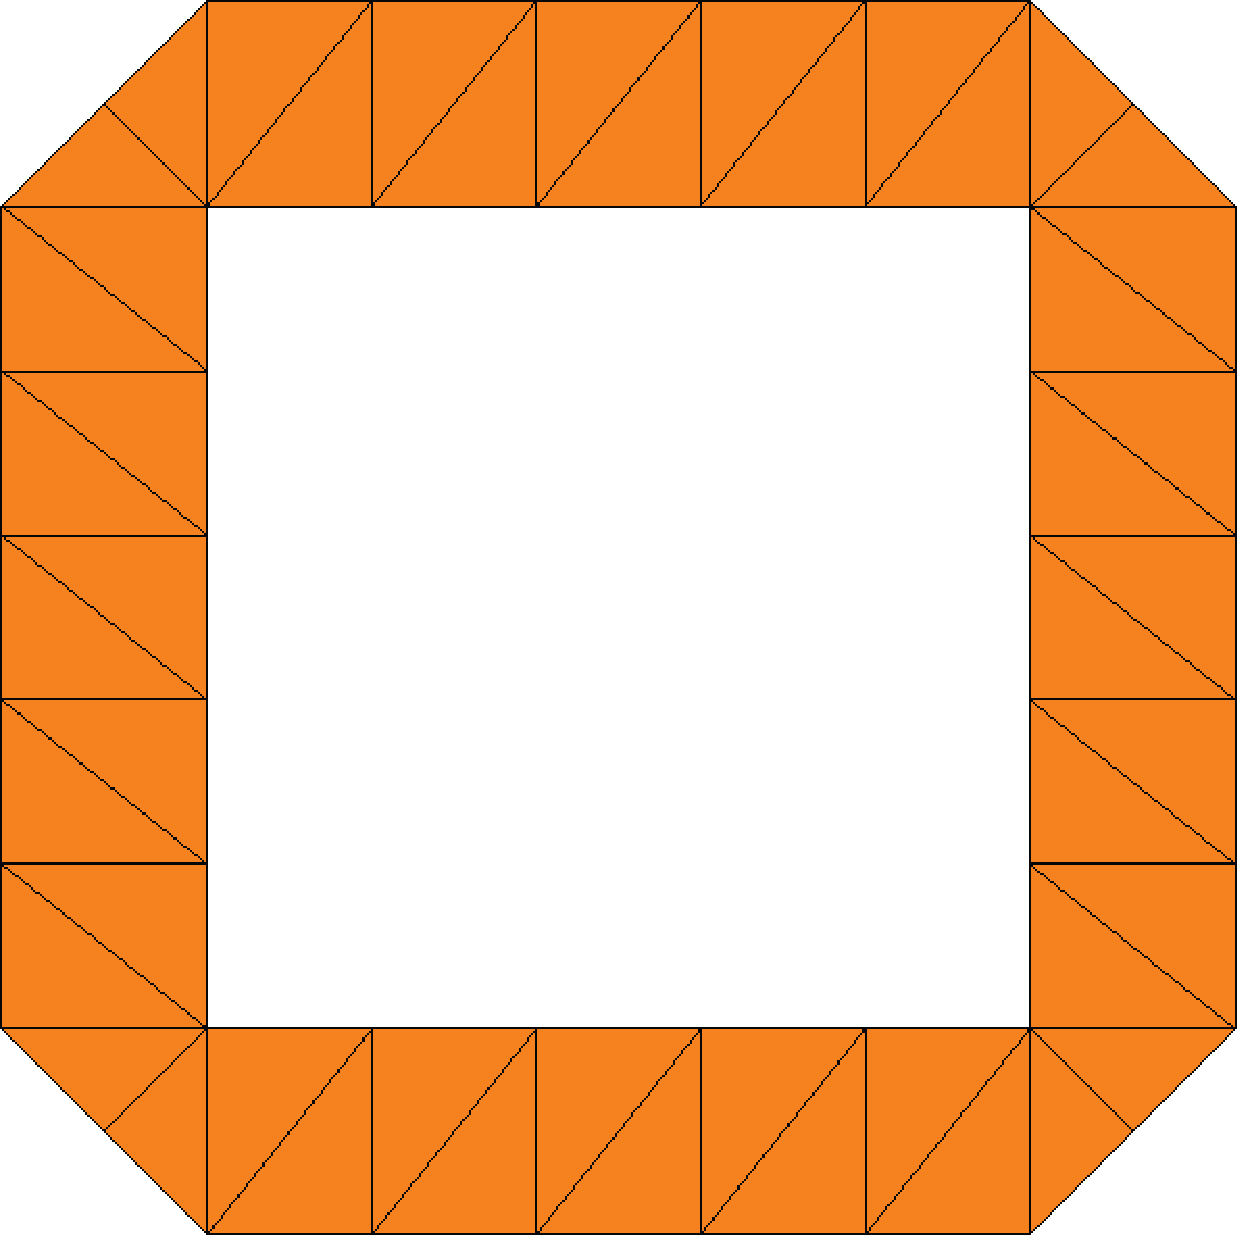
\includegraphics[width=0.3\textwidth]{Images/inflation_3.pdf}
\hspace{\fill}
\pause 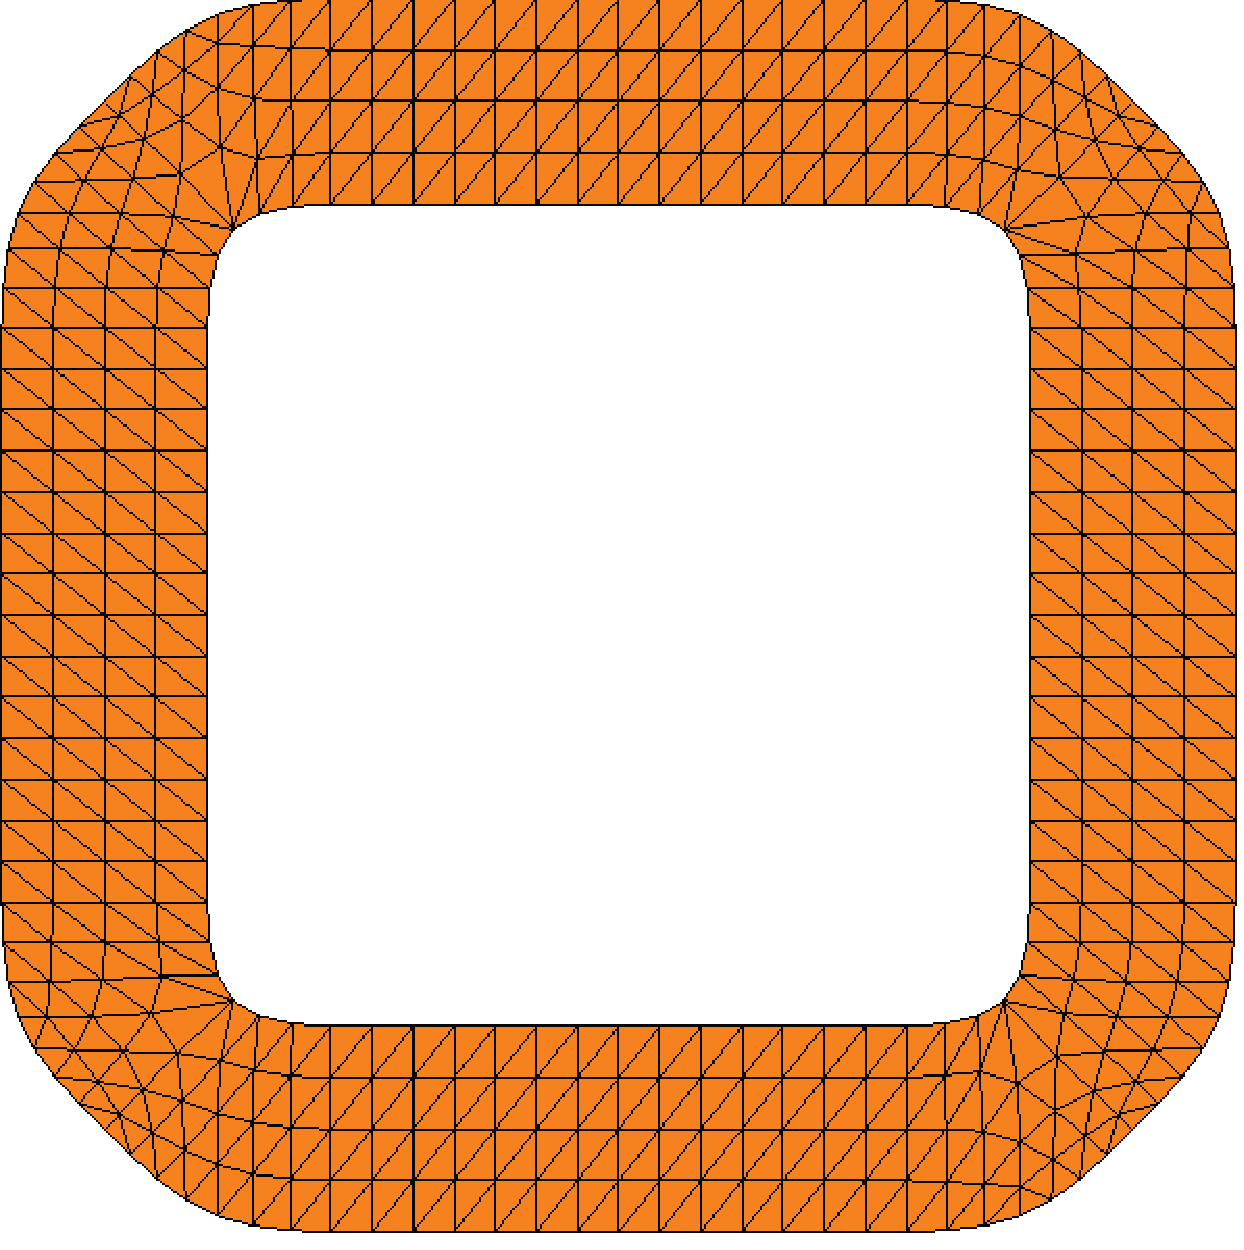
\includegraphics[width=0.3\textwidth]{Images/inflation_4.pdf}
\hspace{\fill}
\end{figure}
\end{frame}

\begin{frame}{Periodic inflation}
% Periodic inflation example
\begin{figure}
\hspace{\fill}
\includegraphics[width=0.4\textwidth]{Images/brick5_periodic.png}
\hspace{\fill}
\includegraphics[width=0.4\textwidth]{Images/star_periodic.png}
\hspace{\fill}

\vspace{3mm}
\hspace{\fill}
\includegraphics[width=0.4\textwidth]{Images/truncated_octahedron_periodic.png}
\hspace{\fill}
\includegraphics[width=0.4\textwidth]{Images/diamond_periodic.png}
\hspace{\fill}
\end{figure}
\end{frame}

\begin{frame}{Pattern parameters}
% Pattern parameters
\begin{figure}
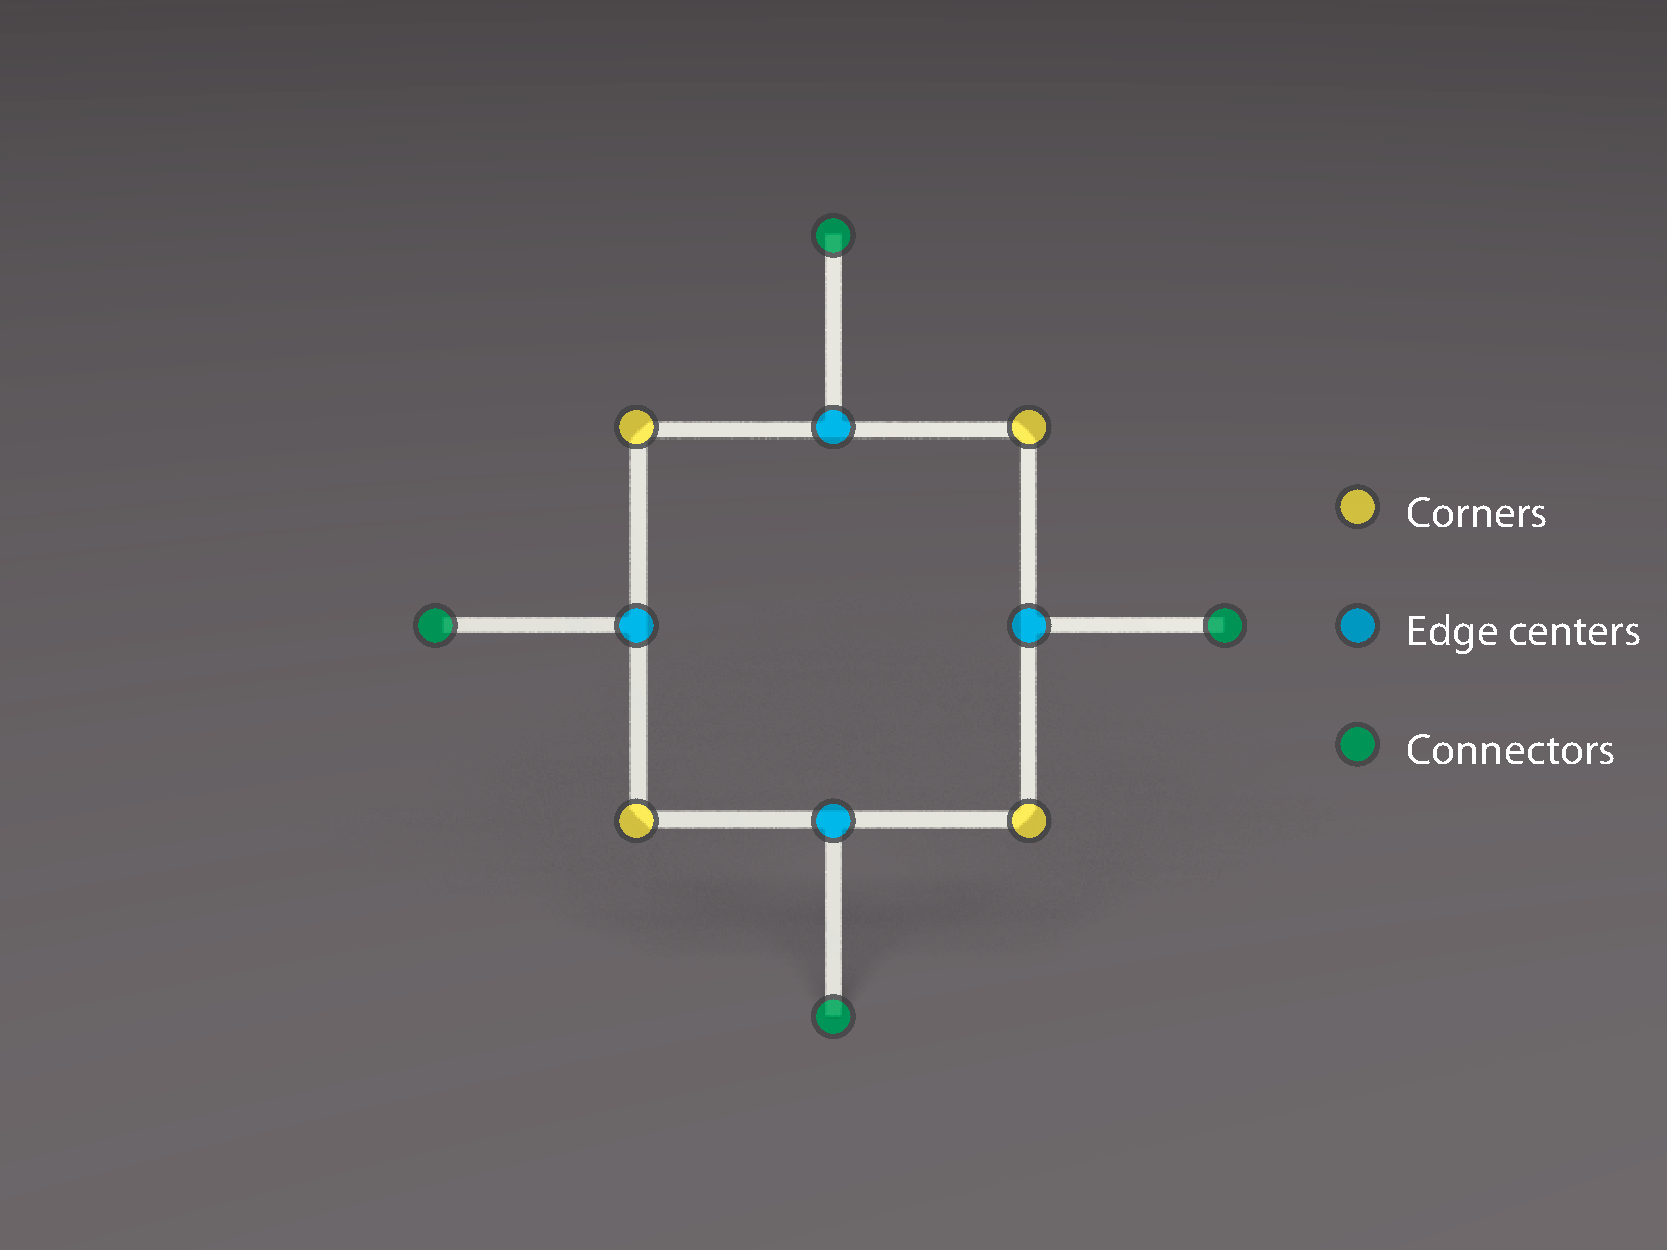
\includegraphics[width=0.9\textwidth]{Images/box_2D_parameters.pdf}
\end{figure}
\end{frame}

\begin{frame}{Pattern parameters}
\begin{figure}
\hspace{\fill}
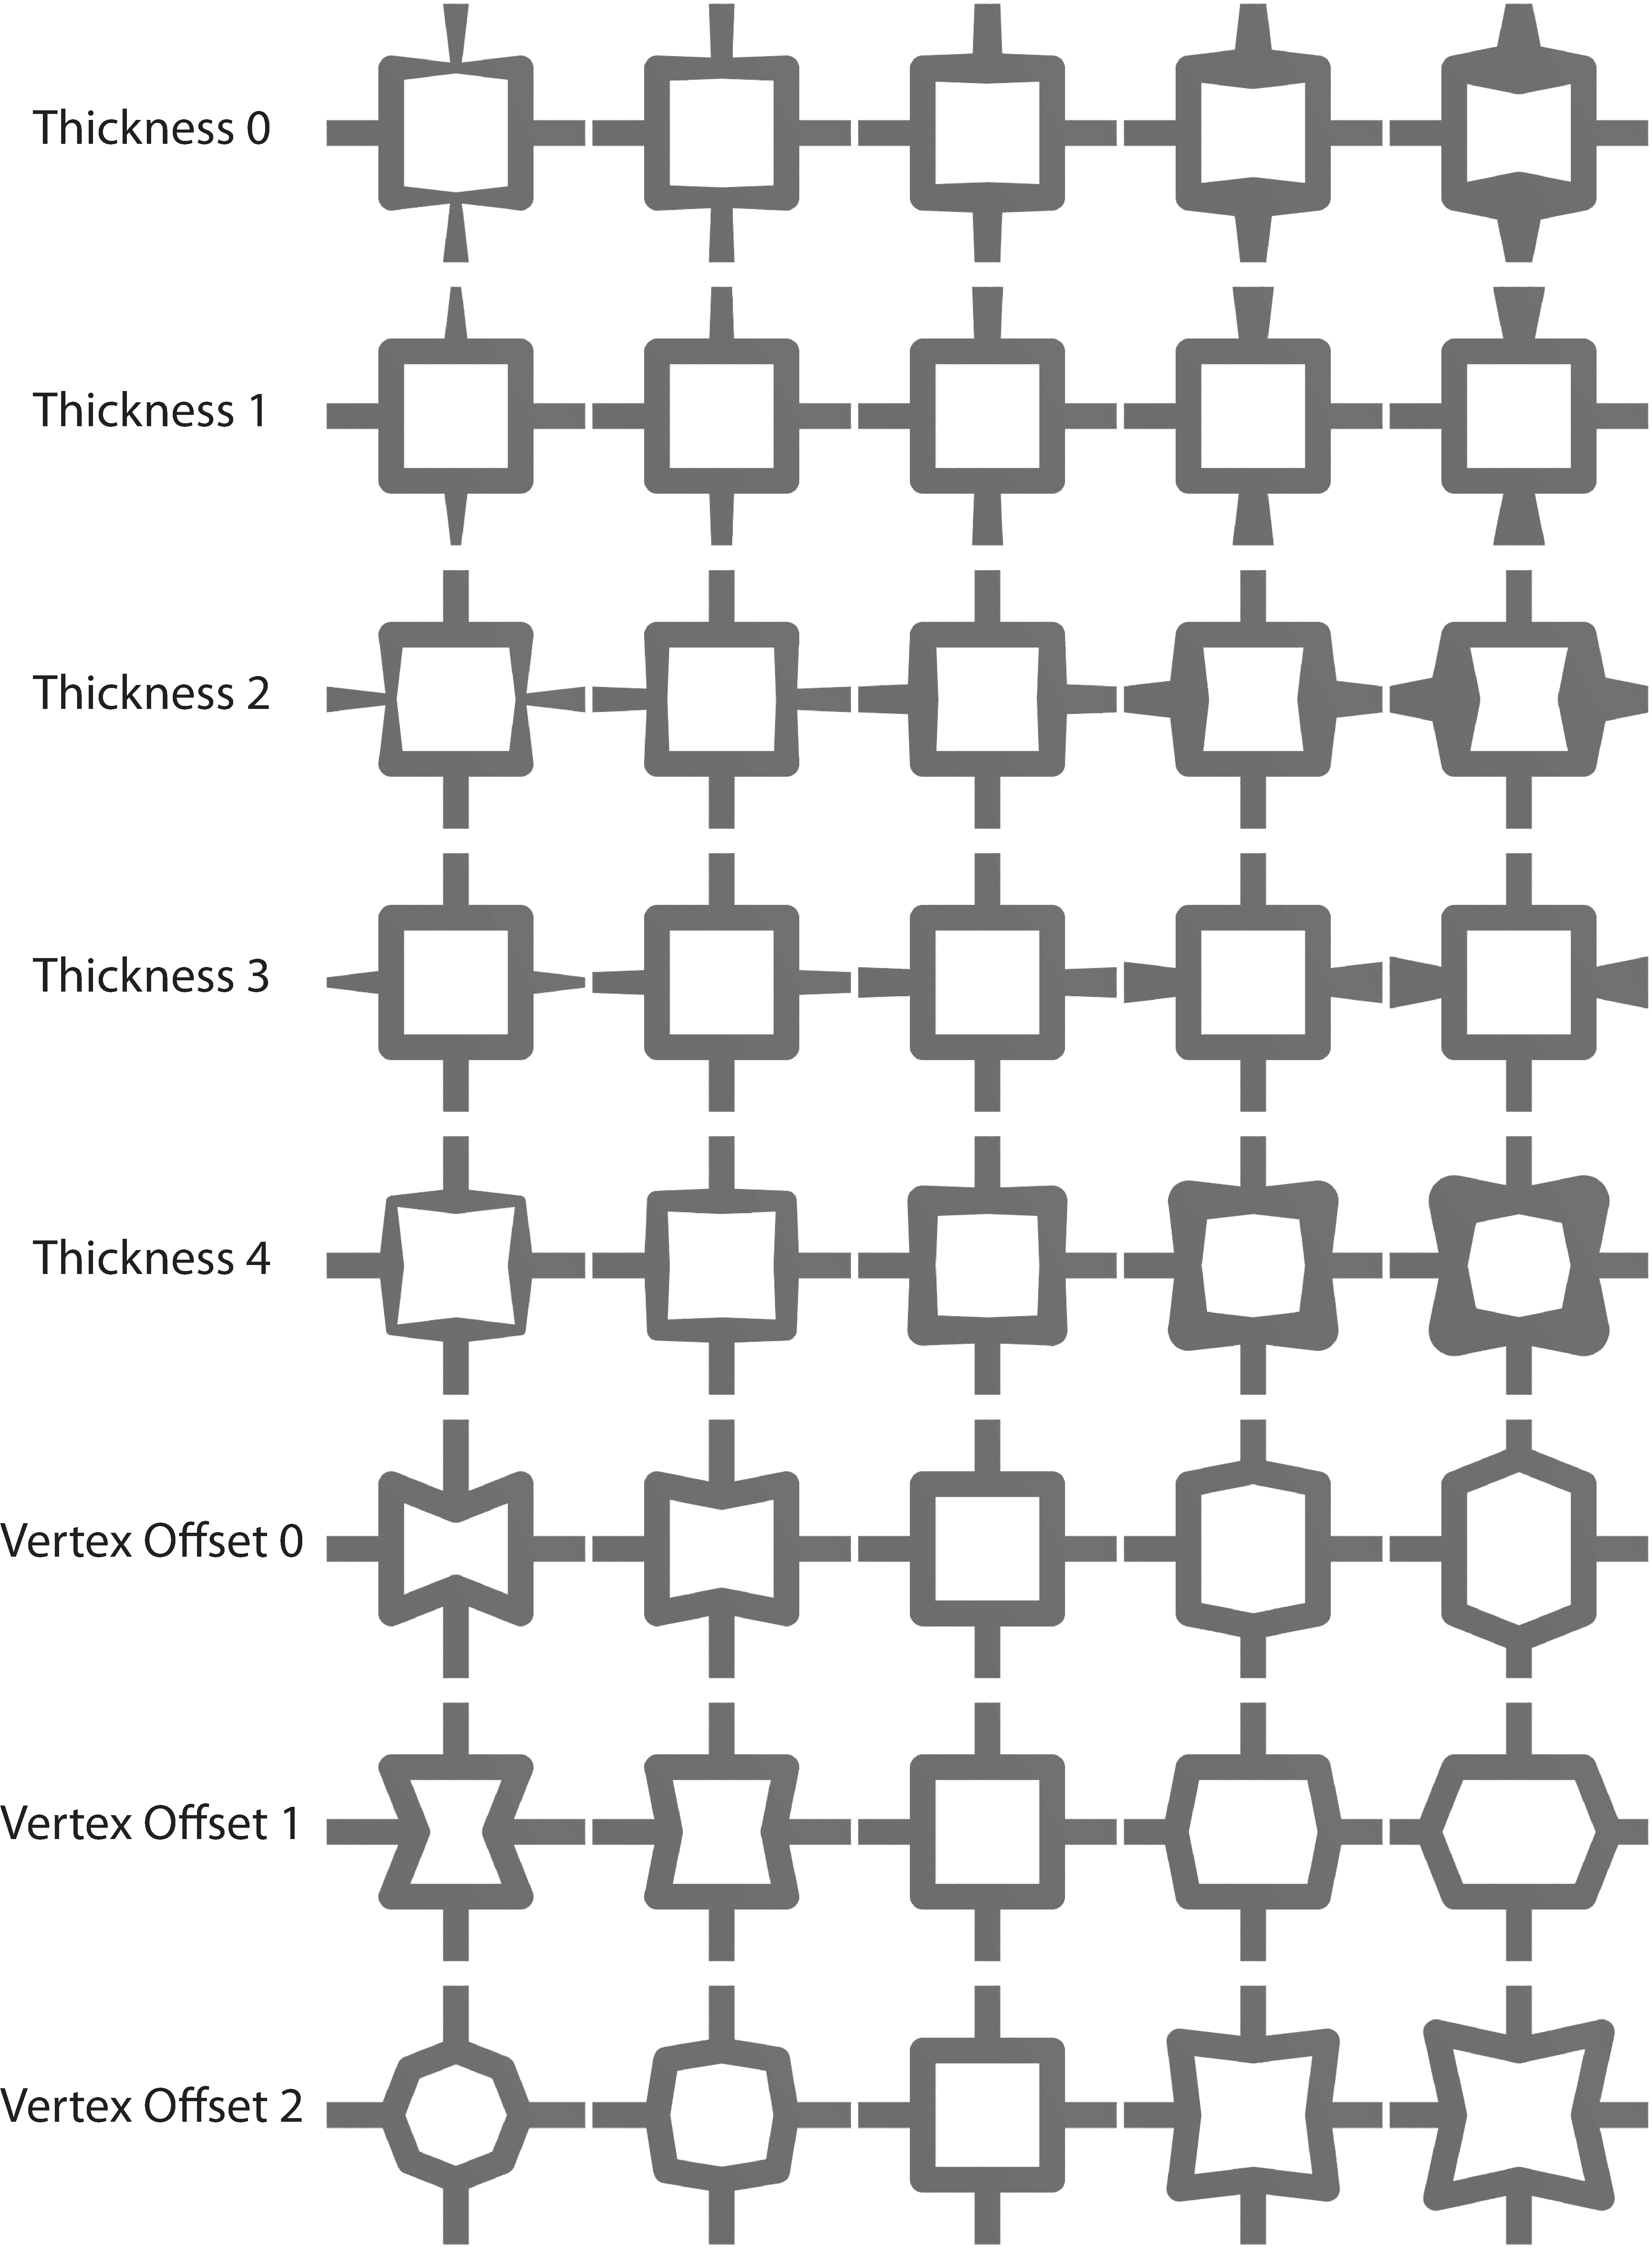
\includegraphics[height=0.8\textheight]{Images/box_2D_param.pdf}
\hspace{\fill}
\end{figure}
\end{frame}

%\begin{frame}{Pattern parameters}
%% Pattern parameters
%\begin{figure}
%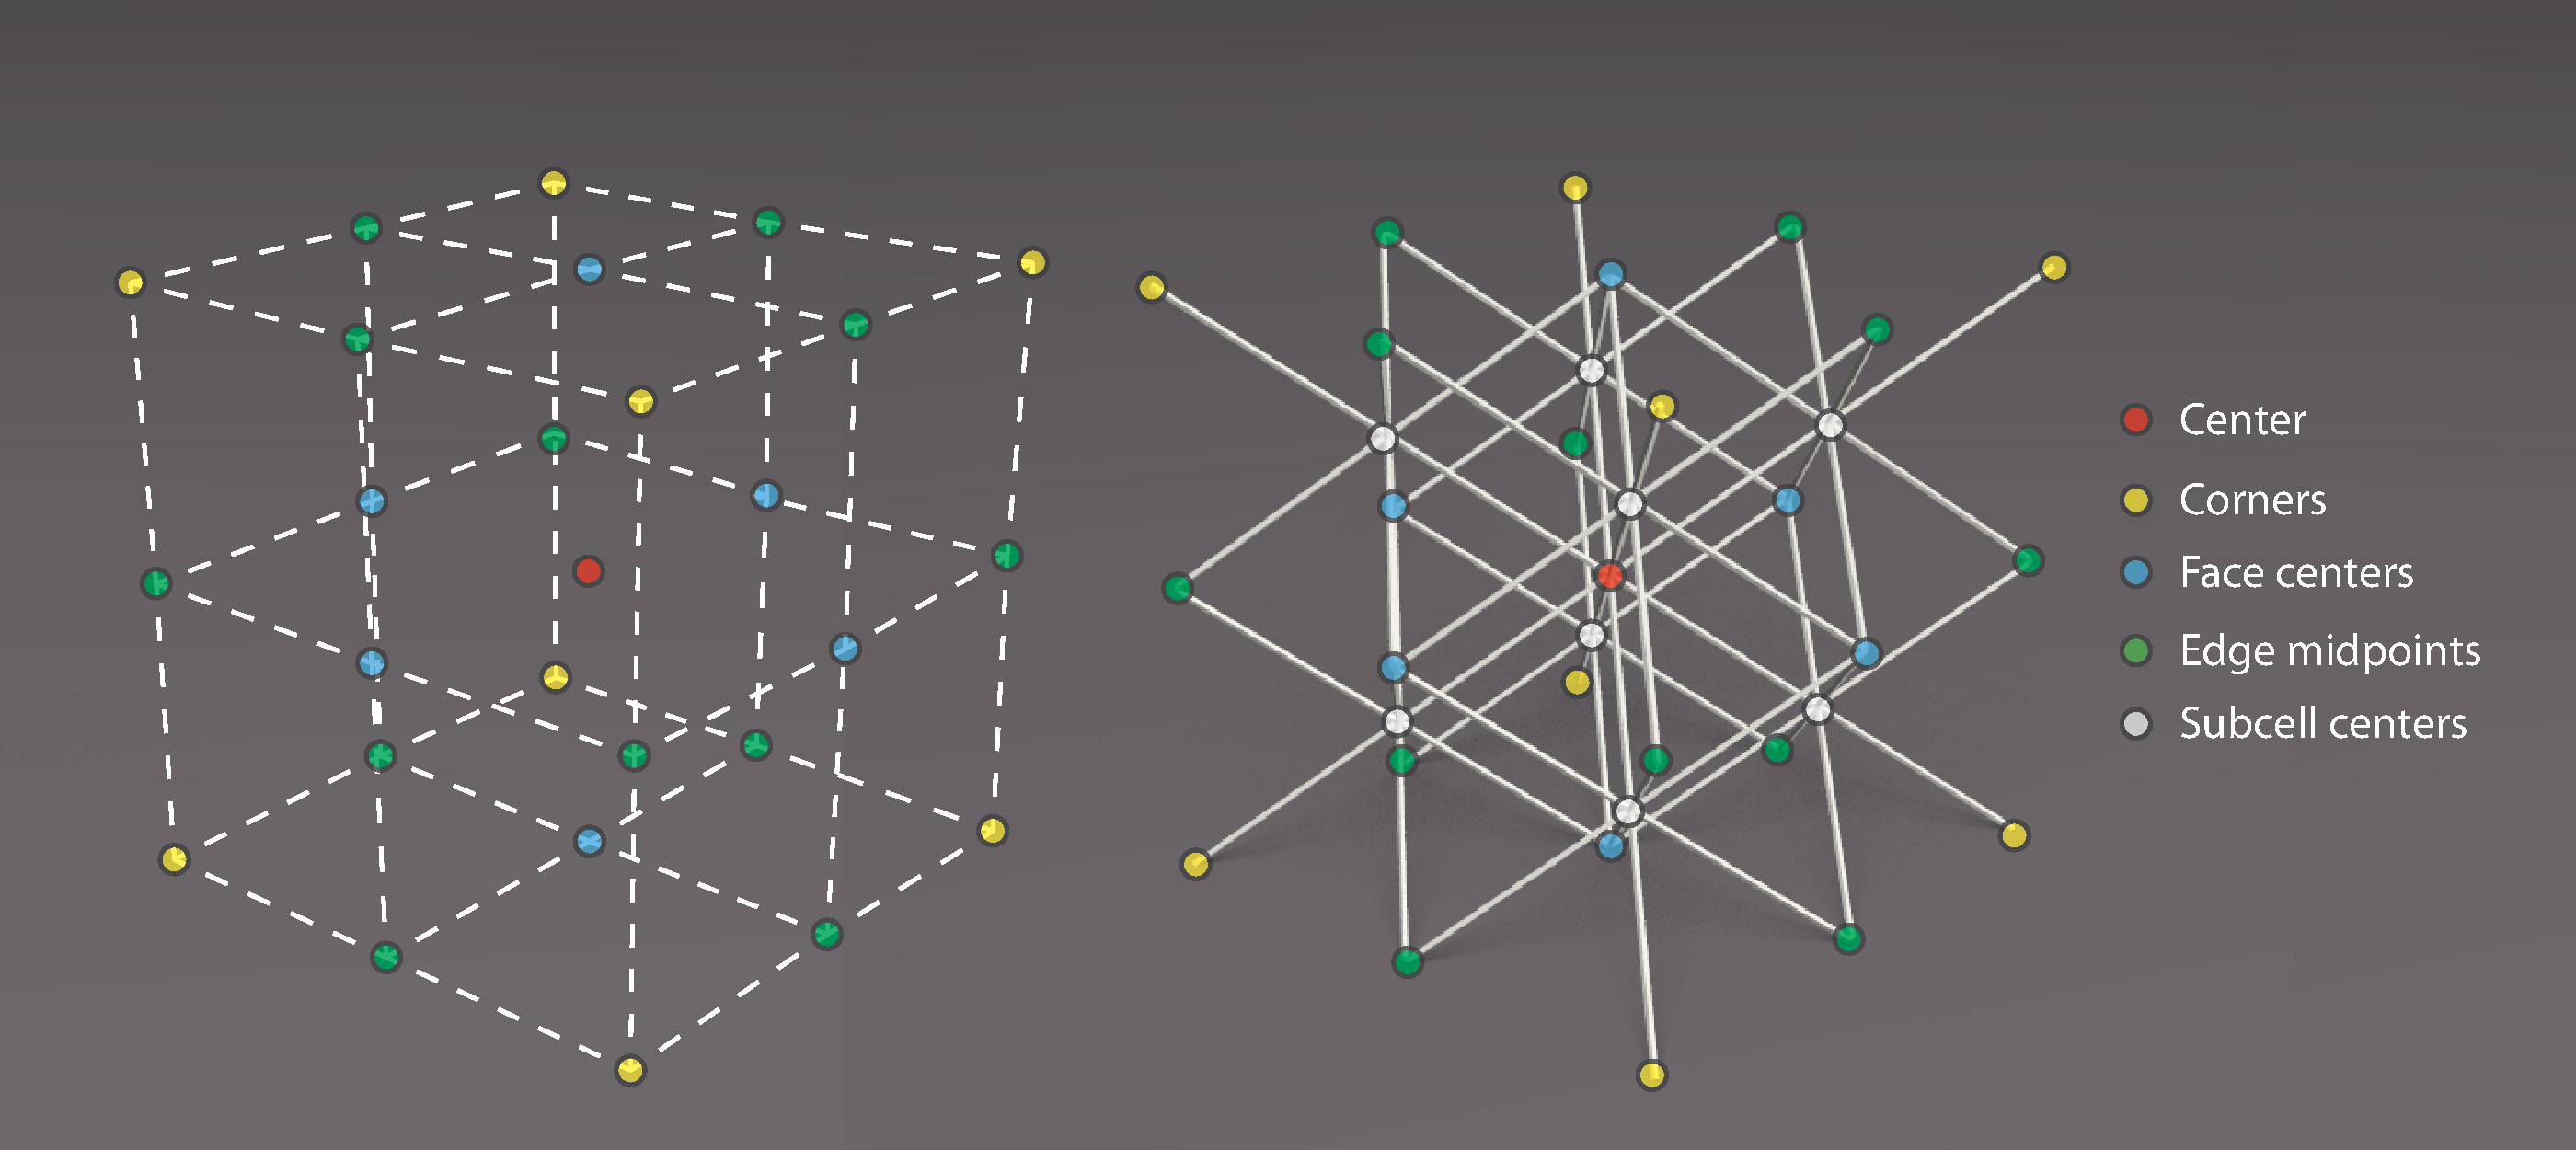
\includegraphics[width=0.9\textwidth]{Images/star_parameters.pdf}
%\end{figure}
%\end{frame}

\begin{frame}{Pattern parameters}
% Pattern parameters
\begin{figure}
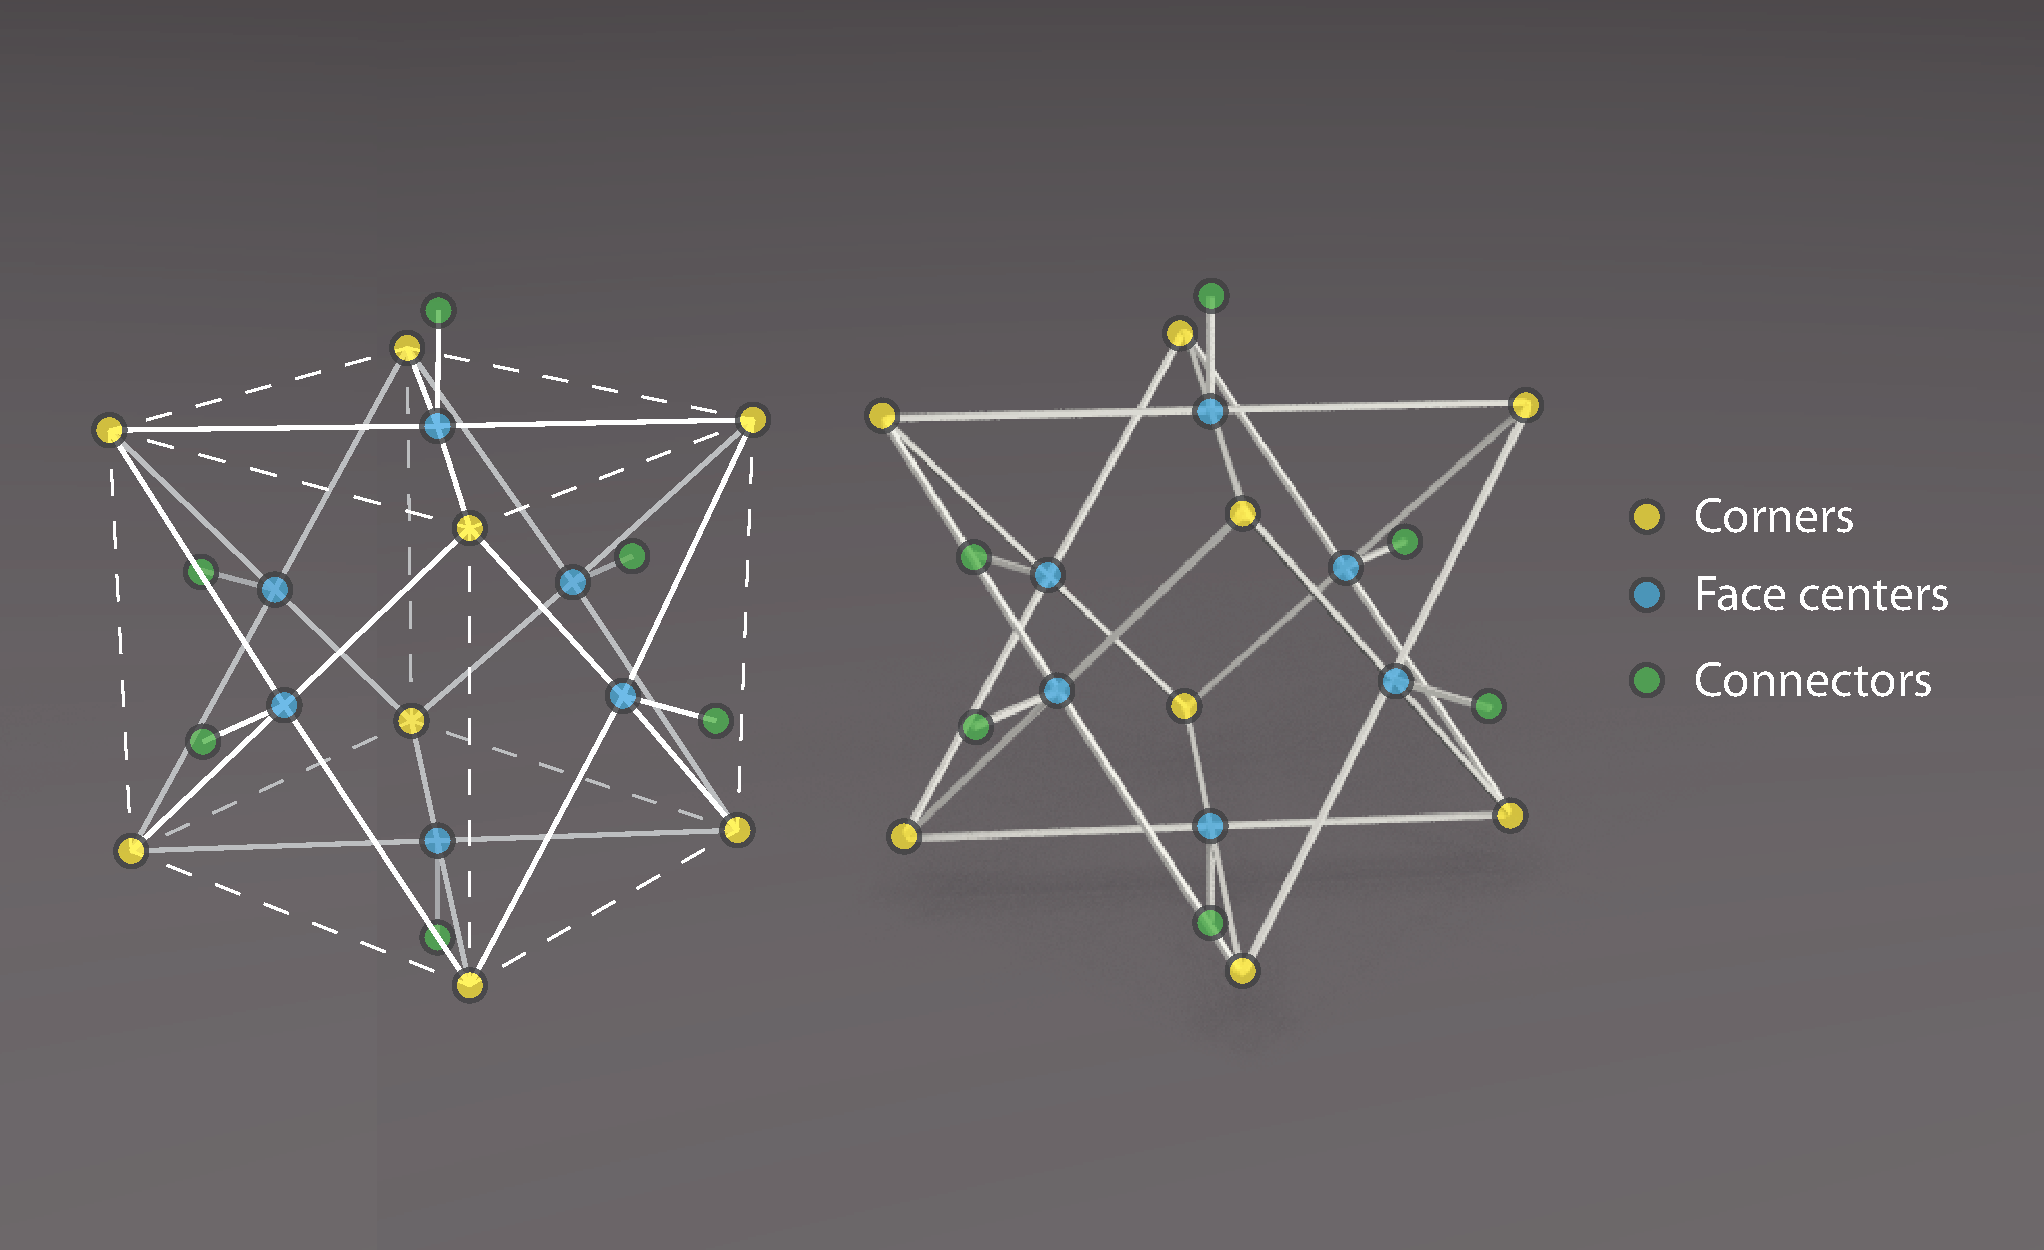
\includegraphics[width=0.9\textwidth]{Images/brick5_parameters.pdf}
\end{figure}
\end{frame}


\begin{frame}{Pattern parameters}
\begin{figure}
\hspace{\fill}
\includegraphics[width=0.9\textwidth]{Images/brick5_param.png}
\hspace{\fill}
\end{figure}
\end{frame}

\begin{frame}{Printibility}
Support structure is bad.
\begin{figure}
\includegraphics[width=0.95\textwidth]{Images/microstructure_support.png}
\end{figure}
\end{frame}

\begin{frame}{Printibility}
Pushing printers to its limit.
\begin{figure}
\includegraphics[height=0.8\textheight]{Images/microstructure_prints.pdf}
\end{figure}
\end{frame}


\section{Pattern Optimization}
\begin{frame}{Goal}
    \begin{itemize}
        \item For each grid cell, find a pattern with $Y, \nu \approx Y^*, \nu^*$ from
   material optimization.
 \item I.e. "invert" the homogenization procedure
 \item Could sample the 9+ dimensional pattern parameter space and find closest
   tensor...
 \item .. but space is huge, $N^P$ sample points ($N$ samples per param, $P$ params)
\end{itemize}
\end{frame}

\begin{frame}{Shape Optimization}
    \begin{itemize}
\item Ideally we can tune the elasticity tensor with an optimization:
    $$ \min_p \norm{C - C^*}^2 $$
\item $p$ controls {\bf shape} of microstructure! How can we optimize it?
\item Use the ``shape derivative''
    \begin{figure}
        \includegraphics[width=.35\textwidth]{Images/vn.pdf}
        $v_n$
    \end{figure}
        $$ J(\omega) = \norm{C(\omega) - C^*}^2 $$
        $$
        \delta J[v_n](\omega) = \lim_{\epsilon \to 0} \frac{J(\omega) - J(\omega_{\text{perturbed by $\epsilon v_n$}})}{\epsilon}
        $$
    \end{itemize}
\end{frame}

\begin{frame}{Shape Optimization}
    \begin{itemize}
        \item Amazingly, the closed form of each entry of the homogenized elasticity tensor can be
              shape differentiated
                $$
                \delta C^H_{ijkl}[v_n] = \frac{1}{|Y|} \int_{\partial \omega} \left[(e^{ij} + e({\bf w}^{ij})) : C : (e^{kl} + e({\bf w}^{kl}))\right] v_n \dA({\bf y})
                $$
            \item If we know the normal velocity caused by each pattern parameter, $p_a$, plug it in (chain rule):
              $$
              \pder{C^H_{ijkl}}{p_a} =
              \frac{1}{|Y|} \int_{\partial \omega} \left[(e^{ij} + e({\bf w}^{ij})) : C : (e^{kl} + e({\bf w}^{kl}))\right] {\bf v}_{p_a} \cdot {\bf \hat{n}} \dA({\bf y})
              $$
    \end{itemize}
\end{frame}

\begin{frame}{Other Objectives}
    \begin{itemize}
        \item It might be better to optimize a different objective than fitting the elasticity tensor.
        \begin{itemize}
            \item Fit compliance tensor
                $$ min_p \norm{C^{-1} - {C^*}^{-1}}^2 $$
            \item Fit Poisson ratio
                $$ min_p \norm{\nu - \nu^*}^2 $$
        \end{itemize}
        \item Gradients of these can be computed using chain rule.
    \end{itemize}
\end{frame}

\begin{frame}{Example}
\end{frame}


\end{document}
